\documentclass[11pt]{article}
\usepackage[a4paper,margin=1in]{geometry}
\usepackage{amsmath,amssymb}
\usepackage{graphicx}
\usepackage{booktabs}
\usepackage{float}
\usepackage{array}
\usepackage{hyperref}

\title{Offline Coefficient-Space Comparison for Case-2 Maps\\ANN vs GPR, $n_s\in\{131,141,151\}$}
\author{Sebastian Ares de Parga Regalado}
\date{\today}

\begin{document}
\maketitle

\section*{Objective}
This report compares six previously trained Case-2 maps in pure offline reconstruction mode:
\[
(\mu,t)\mapsto q_s(\mu,t),
\]
without running online nonlinear ROM solves.

The compared models include ANN and GPR maps with
\[
n_s\in\{131,141,151\},
\]
using the same linear PROM reference trajectories.

Reference trajectories are the linear PROM coefficients $q_N^{lin}(t;\mu)$ with $n_{tot}=151$ at
\[
\mu^{(v)}=(4.875,0.0225),\quad
\mu^{(1)}=(4.560,0.0190),\quad
\mu^{(2)}=(5.190,0.0260).
\]


\section*{Model specifications used in this report}
All maps use inputs $(\mu_1,\mu_2,t)$. ANN131/ANN141 output $q_s$; ANN151 outputs the full $q_N$.
For ANN151, the hidden architecture is the same as in the training script core MLP:
\[
(32,64,128,256,256)\ \text{with ELU activations}.
\]

\begin{table}[H]
\centering
\caption{ANN training setup (from Stage-3 summaries).}
\scriptsize
\begin{tabular}{ccccccccc}
\toprule
$n_s$ & hidden dims & act. & drop. & batch & lr & weight decay & epochs ran & best val MSE \\
\midrule
131 & \texttt{(32, 64, 128, 256, 256)} & elu & 0.0 & 128 & \texttt{0.001} & \texttt{1e-06} & 1297 & \texttt{0.2420964539051056} \\
141 & \texttt{(32, 64, 128, 256, 256)} & elu & 0.0 & 128 & \texttt{0.001} & \texttt{1e-06} & 2000 & \texttt{0.1521771103143692} \\
151 & \texttt{(32, 64, 128, 256, 256)} & elu & 0.0 & 128 & \texttt{1e-3} & \texttt{1e-6} & 2000 & \texttt{0.3817078769207001} \\
\bottomrule
\end{tabular}
\end{table}

\begin{table}[H]
\centering
\caption{GPR kernels after optimization, including WhiteKernel terms.}
\scriptsize
\begin{tabular}{cp{0.20\textwidth}p{0.25\textwidth}cccc}
\toprule
$n_s$ & kernel init & kernel learned & $\alpha$ & WhiteK & WhiteK bounds & val rel. Frobenius (\%) \\
\midrule
131 & \texttt{1**2 * Matern(length\_scale=[1, 1, 1], nu=1.5) + WhiteKernel(noise\_level=1e-06)} & \texttt{2.67**2 * Matern(length\_scale=[0.0001, 0.0001, 0.146], nu=1.5) + WhiteKernel(noise\_level=1e-10)} & \texttt{1e-12} & True & \texttt{(1e-10, 1.0)} & \texttt{0.9932419125450657} \\
141 & \texttt{1**2 * Matern(length\_scale=[1, 1, 1], nu=1.5) + WhiteKernel(noise\_level=1e-06)} & \texttt{5.01**2 * Matern(length\_scale=[0.0001, 6.39, 0.236], nu=1.5) + WhiteKernel(noise\_level=1e-10)} & \texttt{1e-12} & True & \texttt{(1e-10, 1.0)} & \texttt{0.420604737643367} \\
151 & \texttt{1**2 * Matern(length\_scale=[1, 1, 1], nu=1.5) + WhiteKernel(noise\_level=1e-06)} & \texttt{4.86**2 * Matern(length\_scale=[0.0001, 6.42, 0.237], nu=1.5) + WhiteKernel(noise\_level=1e-10)} & \texttt{1e-12} & True & \texttt{(1e-10, 1.0)} & \texttt{0.0899985346079204} \\
\bottomrule
\end{tabular}
\end{table}


\section*{Error definitions}
For a model with split $n_{tot}=n_p+n_s$, we compare predicted secondary coefficients against the corresponding tail of the linear reference:
\[
q_s^{ref}(t;\mu)=\big[q_N^{lin}(t;\mu)\big]_{n_p+1:n_{tot}},
\qquad
q_s^{pred}(t;\mu)=\mathcal M_{\theta}(\mu,t).
\]
For each predicted coefficient index $i=1,\dots,n_s$:
\[
E_i^{abs}(\mu)=\left\|q_{s,i}^{ref}-q_{s,i}^{pred}\right\|_2,
\qquad
E_i^{rel}(\mu)=100\,
\frac{\left\|q_{s,i}^{ref}-q_{s,i}^{pred}\right\|_2}
{\left\|q_{s,i}^{ref}\right\|_2+\varepsilon}.
\]
Global secondary-trajectory error:
\[
E_F(\mu)=100\,
\frac{\left\|Q_s^{ref}-Q_s^{pred}\right\|_F}
{\left\|Q_s^{ref}\right\|_F+\varepsilon}.
\]

Since models have different $n_s$, each curve starts at global index $n_p+1$ with $n_p=n_{tot}-n_s$.
Therefore, missing lower global indices for some curves are expected.

\section*{Pointwise summary}
\begin{table}[H]
\centering
\caption{Offline coefficient errors per point (\%).}
\begin{tabular}{lccccc}
\toprule
Model & $n_s$ & $E_F$ & mean$(E_i^{rel})$ & p95$(E_i^{rel})$ & max$(E_i^{rel})$ \\
\midrule
\multicolumn{6}{c}{\(\mu=(4.875,0.0225)\)} \\
\midrule
ANN & 131 & 11.020 & 27.578 & 64.427 & 77.394 \\
ANN & 141 & 4.968 & 17.719 & 40.772 & 51.943 \\
ANN & 151 & 1.791 & 30.688 & 79.297 & 87.480 \\
GPR & 131 & 0.562 & 1.313 & 4.746 & 5.443 \\
GPR & 141 & 0.162 & 0.669 & 3.060 & 3.842 \\
GPR & 151 & 0.034 & 0.624 & 2.987 & 3.841 \\
\midrule
\multicolumn{6}{c}{\(\mu=(4.560,0.0190)\)} \\
\midrule
ANN & 131 & 102.964 & 142.204 & 201.576 & 272.048 \\
ANN & 141 & 9.206 & 27.858 & 59.705 & 78.524 \\
ANN & 151 & 3.842 & 49.200 & 101.068 & 118.742 \\
GPR & 131 & 100.027 & 100.004 & 100.053 & 100.383 \\
GPR & 141 & 100.004 & 100.001 & 100.071 & 100.383 \\
GPR & 151 & 100.200 & 100.006 & 100.103 & 100.408 \\
\midrule
\multicolumn{6}{c}{\(\mu=(5.190,0.0260)\)} \\
\midrule
ANN & 131 & 69.570 & 113.381 & 170.202 & 201.128 \\
ANN & 141 & 10.268 & 33.535 & 64.266 & 80.333 \\
ANN & 151 & 5.474 & 53.547 & 105.780 & 138.958 \\
GPR & 131 & 99.987 & 100.003 & 100.046 & 100.083 \\
GPR & 141 & 99.998 & 100.005 & 100.057 & 100.171 \\
GPR & 151 & 99.892 & 100.003 & 100.061 & 100.171 \\
\midrule
\bottomrule
\end{tabular}
\end{table}

\section*{Average over the three points}
\begin{table}[H]
\centering
\caption{Averaged offline coefficient errors over the three points (\%).}
\begin{tabular}{lccccc}
\toprule
Model & $n_s$ & mean $E_F$ & mean(mean$(E_i^{rel})$) & mean(p95$(E_i^{rel})$) & mean(max$(E_i^{rel})$) \\
\midrule
ANN & 131 & 61.185 & 94.387 & 145.402 & 183.523 \\
ANN & 141 & 8.147 & 26.371 & 54.914 & 70.267 \\
ANN & 151 & 3.702 & 44.479 & 95.382 & 115.060 \\
GPR & 131 & 66.859 & 67.107 & 68.282 & 68.636 \\
GPR & 141 & 66.721 & 66.892 & 67.729 & 68.132 \\
GPR & 151 & 66.709 & 66.878 & 67.717 & 68.140 \\
\bottomrule
\end{tabular}
\end{table}

\section*{Per-coefficient curves}
\begin{figure}[H]
\centering

\includegraphics[width=0.96\textwidth]{Figures/case2_ann_gpr_coeff_offline/mu1_4.875_mu2_0.0225_coeff_abs_rel_vs_global_index_ann_gpr_131_141_151.png}
\caption{Absolute and relative coefficient errors vs global coefficient index at $\mu^{(v)}=(4.875,0.0225)$.}
\end{figure}

\begin{figure}[H]
\centering

\includegraphics[width=0.96\textwidth]{Figures/case2_ann_gpr_coeff_offline/mu1_4.560_mu2_0.0190_coeff_abs_rel_vs_global_index_ann_gpr_131_141_151.png}
\caption{Absolute and relative coefficient errors vs global coefficient index at $\mu^{(1)}=(4.560,0.0190)$.}
\end{figure}

\begin{figure}[H]
\centering

\includegraphics[width=0.96\textwidth]{Figures/case2_ann_gpr_coeff_offline/mu1_5.190_mu2_0.0260_coeff_abs_rel_vs_global_index_ann_gpr_131_141_151.png}
\caption{Absolute and relative coefficient errors vs global coefficient index at $\mu^{(2)}=(5.190,0.0260)$.}
\end{figure}

\section*{GPR zoom}
\begin{figure}[H]
\centering

\includegraphics[width=0.92\textwidth]{Figures/case2_ann_gpr_coeff_offline/mu1_4.875_mu2_0.0225_gpr_rel_zoom_ann_gpr_131_141_151.png}
\caption{Zoomed GPR comparison at $\mu^{(v)}=(4.875,0.0225)$, including pairwise differences.}
\end{figure}

\begin{figure}[H]
\centering

\includegraphics[width=0.92\textwidth]{Figures/case2_ann_gpr_coeff_offline/mu1_4.560_mu2_0.0190_gpr_rel_zoom_ann_gpr_131_141_151.png}
\caption{Zoomed GPR comparison at $\mu^{(1)}=(4.560,0.0190)$, including pairwise differences.}
\end{figure}

\begin{figure}[H]
\centering

\includegraphics[width=0.92\textwidth]{Figures/case2_ann_gpr_coeff_offline/mu1_5.190_mu2_0.0260_gpr_rel_zoom_ann_gpr_131_141_151.png}
\caption{Zoomed GPR comparison at $\mu^{(2)}=(5.190,0.0260)$, including pairwise differences.}
\end{figure}

\section*{Hybrid state-space overlays (HDM comparison)}
Using the same predicted coefficients, hybrid full reduced trajectories were built as
\[
q_N^{hyb}=
\begin{bmatrix}
q_p^{lin}\\ q_s^{pred}
\end{bmatrix},
\]
with $(n_p,n_s)=(20,131)$, $(10,141)$, and $(0,151)$ depending on the model.
Then states were reconstructed by
\[
u^{hyb}(t)=u_{ref}+V_{tot}q_N^{hyb}(t),
\]
and compared directly against HDM snapshots.

\begin{table}[H]
\centering
\caption{Hybrid state errors per point (\%).}
\begin{tabular}{lccc}
\toprule
Model & $n_s$ & err.\ vs HDM (\%) & err.\ vs linear state (\%) \\
\midrule
\multicolumn{4}{c}{\(\mu=(4.875,0.0225)\)} \\
\midrule
ANN & 131 & 0.633 & 0.535 \\
ANN & 141 & 0.599 & 0.447 \\
ANN & 151 & 0.849 & 0.769 \\
GPR & 131 & 0.411 & 0.027 \\
GPR & 141 & 0.411 & 0.015 \\
GPR & 151 & 0.411 & 0.015 \\
\midrule
\multicolumn{4}{c}{\(\mu=(4.560,0.0190)\)} \\
\midrule
ANN & 131 & 5.300 & 5.245 \\
ANN & 141 & 0.954 & 0.856 \\
ANN & 151 & 1.714 & 1.669 \\
GPR & 131 & 5.147 & 5.095 \\
GPR & 141 & 9.342 & 9.295 \\
GPR & 151 & 43.544 & 43.525 \\
\midrule
\multicolumn{4}{c}{\(\mu=(5.190,0.0260)\)} \\
\midrule
ANN & 131 & 3.448 & 3.424 \\
ANN & 141 & 1.014 & 0.919 \\
ANN & 151 & 2.441 & 2.405 \\
GPR & 131 & 4.926 & 4.921 \\
GPR & 141 & 8.944 & 8.947 \\
GPR & 151 & 43.879 & 43.886 \\
\midrule
\bottomrule
\end{tabular}
\end{table}

\begin{table}[H]
\centering
\caption{Average hybrid state errors over the three points (\%).}
\begin{tabular}{lccc}
\toprule
Model & $n_s$ & mean err.\ vs HDM (\%) & mean err.\ vs linear state (\%) \\
\midrule
ANN & 131 & 3.127 & 3.068 \\
ANN & 141 & 0.856 & 0.741 \\
ANN & 151 & 1.668 & 1.614 \\
GPR & 131 & 3.495 & 3.348 \\
GPR & 141 & 6.232 & 6.085 \\
GPR & 151 & 29.278 & 29.142 \\
\bottomrule
\end{tabular}
\end{table}

\begin{figure}[H]
\centering
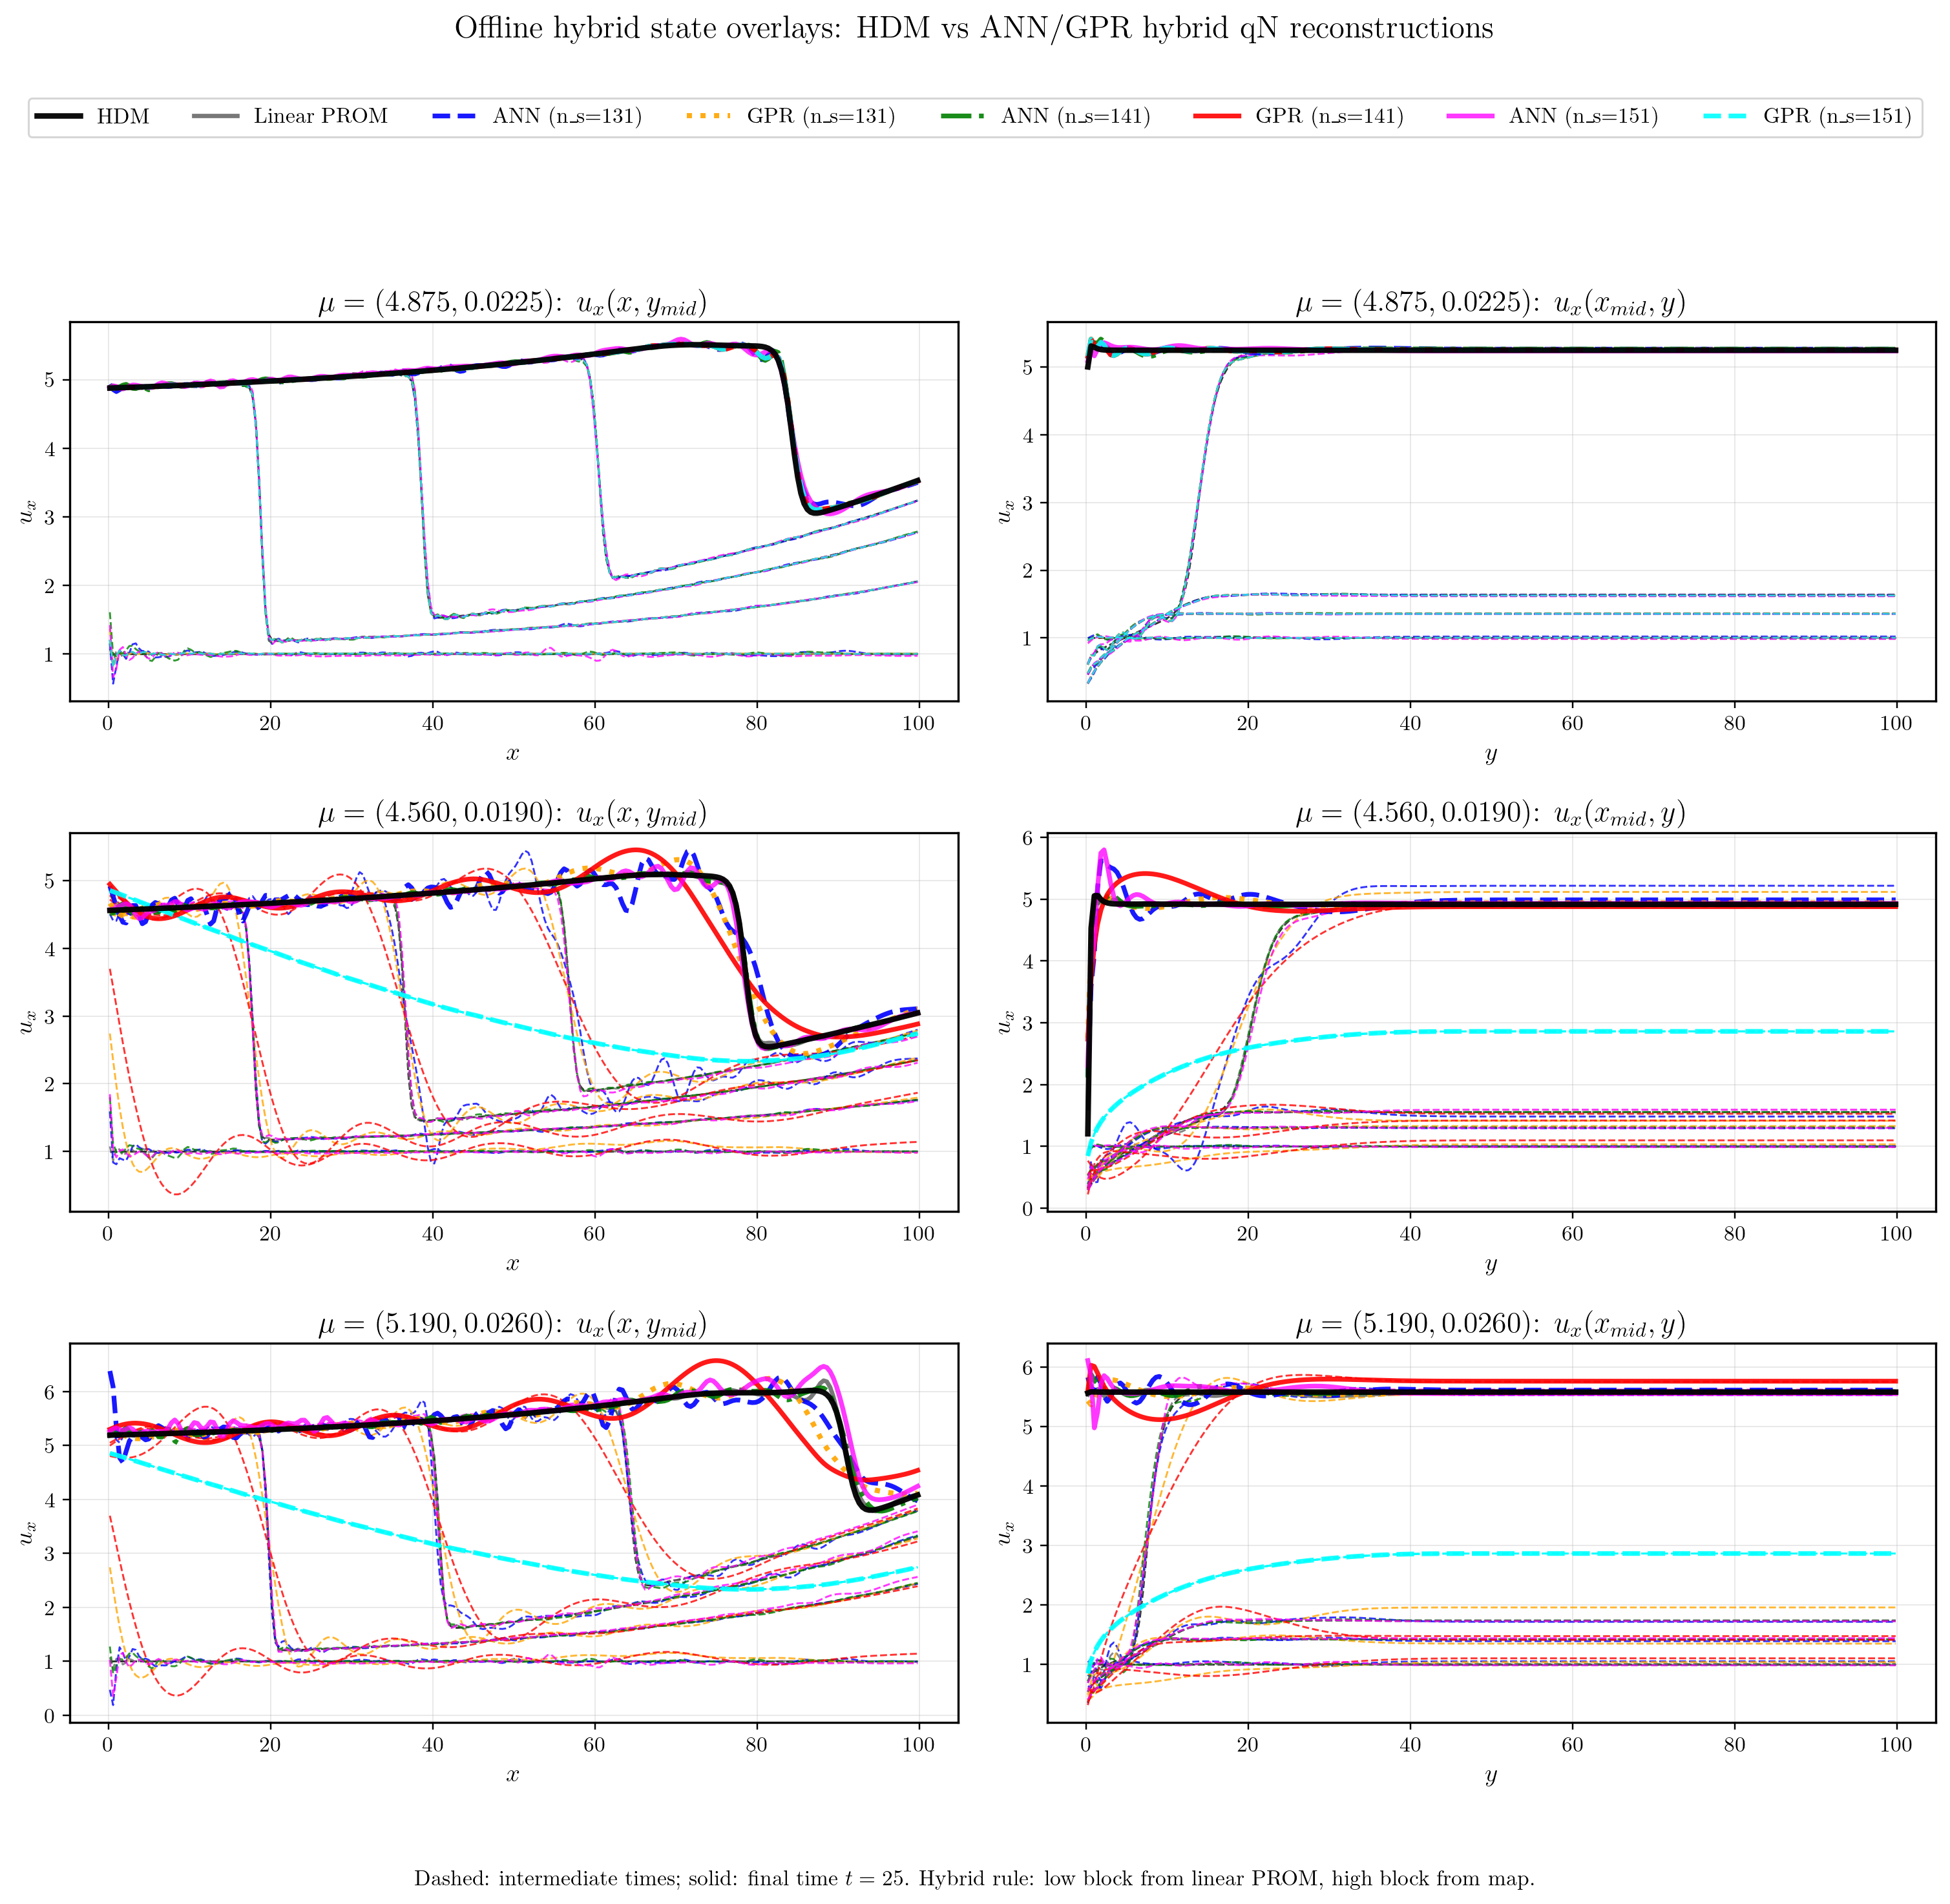
\includegraphics[width=0.98\textwidth]{Figures/case2_ann_gpr_coeff_offline/hybrid_prom_hdm_vs_ann_gpr_models_ann_gpr_131_141_151.png}
\caption{Hybrid offline state overlays: HDM, linear PROM reference, and ANN/GPR hybrid reconstructions for $n_s\in\{131,141,151\}$.}
\end{figure}

\section*{Remarks}
This report is strictly an offline map-comparison diagnostic in coefficient space.
It does not include online ROM reconstruction of state trajectories.

\end{document}
